\chapter{探索我们的环境}\label{ch:g6:exploring-our-environment}

七月的正午穿过校园操场，墙的南面
摸上去烫手，沥青路面上方的空气扭曲晃动，而
目之所及唯一的绿色，是裂缝里的一株杂草。绕到
北墙后面：空气清凉，土壤潮湿，长着\omterm{prop:g4:plants-without-seeds:damp}{苔藓}，石块下躲着鼠妇。
两个世界，相距仅三米。本学年从探索
\omterm{def:g6:exploring-our-environment:components}{环境}开始，像科学家那样——测量\omterm{def:g6:exploring-our-environment:components}{环境}，
并追问每种\omterm{def:g6:exploring-our-environment:components}{生物}为何恰好生活在那里。

\section{环境由什么构成}

\begin{definition}[环境的组成成分]\label{def:g6:exploring-our-environment:components}
一个\emph{环境}\index{环境}——如院子、树林、
池塘岸边——包含三类组成成分：
\begin{enumerate}
  \item \emph{生物}\index{生物}：\omterm{def:g1:animals-around-us:animal}{动物}、
        \omterm{def:g1:plants-around-us:plant}{植物}、蘑菇以及存在的微观生命；
  \item \emph{矿物质}\index{矿物质}，
        \omterm{def:g1:living-or-not:nonliving}{从未有过生命}：岩石、石块、土壤中的无机部分、水、
        空气；
  \item \emph{痕迹和遗骸}：生物的
        枯叶、倒木、粪便、\omterm{def:g1:animals-around-us:covering}{羽毛}、贝壳——
        “曾经有生命”一栏（见
        \cref{def:g1:living-or-not:nonliving}），如今
        成了探索者的线索包。
\end{enumerate}
\end{definition}

\begin{example}[北墙后的清点]\label{ex:g6:exploring-our-environment:inventory}
在阴凉的角落清点十分钟：\omterm{def:g6:exploring-our-environment:components}{生物}——\omterm{prop:g4:plants-without-seeds:damp}{苔藓}、
\omterm{prop:g4:plants-without-seeds:damp}{蕨类}、鼠妇、蜗牛、蜈蚣、常春藤；\omterm{def:g6:exploring-our-environment:components}{矿物质}——墙体的
石块、潮湿的土壤、一洼积水；痕迹——枯
叶、蜗牛壳、墙顶压顶石上的鸟粪。三组清单，
如此，角落便像科学家记录的样地一样得到了描述。
\end{example}

\begin{omfigure}
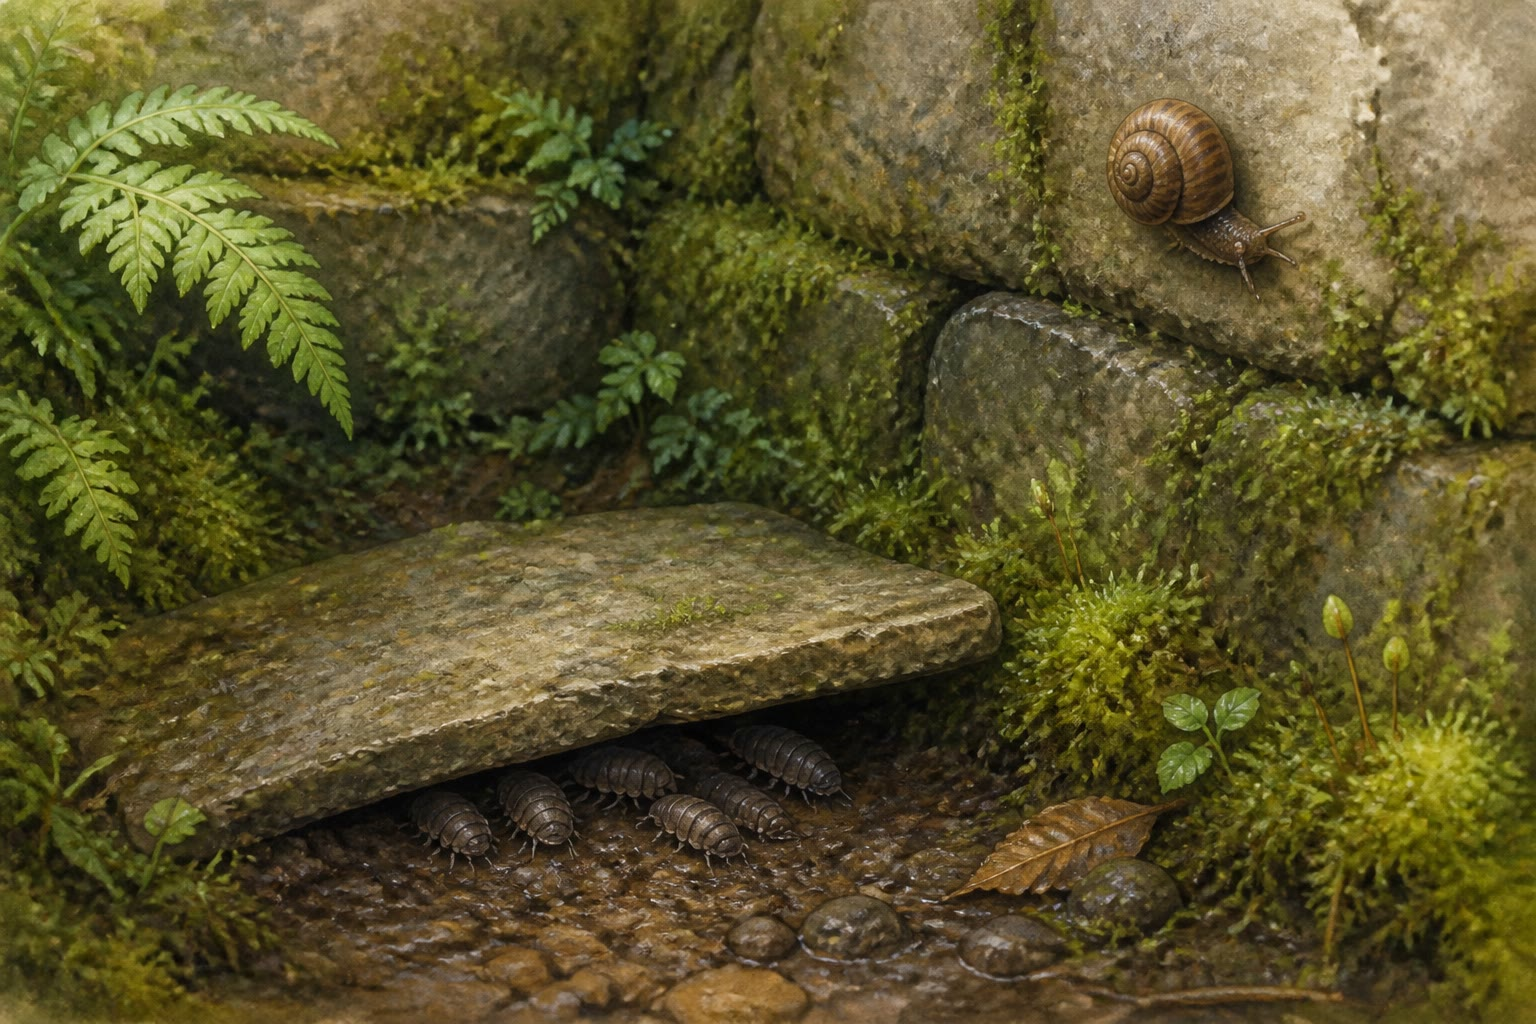
\includegraphics[width=0.62\linewidth]{images/book1/ai/g6-env-wallcorner.jpg}

{\small 阴凉的角落，清点进行中：\omterm{prop:g4:plants-without-seeds:damp}{苔藓}、\omterm{prop:g4:plants-without-seeds:damp}{蕨类}、一只蜗牛
在石头上——掀起的石板下是鼠妇的
\omterm{def:g6:exploring-our-environment:microhabitat}{微生境}（已放回原处）。}
\end{omfigure}

\begin{remark}[痕迹同样是数据]\label{rem:g6:exploring-our-environment:traces}
大多数\omterm{def:g1:animals-around-us:animal}{动物}会躲藏或逃走，因此探索者往往
改为读取\emph{痕迹}：一颗被啃过的榛子能指明林鼠，
蛛网能指明织网者，泥地上的足迹能指明苍鹭。
只记录那些静得足够久、能被看见的\omterm{def:g6:exploring-our-environment:components}{生物}的清单，
会遗漏一半的居民。
\end{remark}

\section{测量环境条件}

\begin{definition}[环境条件]\label{def:g6:exploring-our-environment:conditions}
\omterm{def:g6:exploring-our-environment:components}{环境}的\emph{条件}\index{条件（环境）}是指其可测量的
物理特征：
\begin{itemize}
  \item \emph{温度}\index{温度}，用
        温度计测量，单位为摄氏度；
  \item \emph{湿度}\index{湿度}——空气或
        土壤的潮湿程度；
  \item \emph{光}\index{光（条件）}——从
        全日照到深荫；
\end{itemize}
条件因地点而异——往往在几米之内就
差异明显——并随一天和一年的时间变化。
\end{definition}

\begin{example}[测量后的院子]\label{ex:g6:exploring-our-environment:measured}
七月正午的测量，使用了仪器：南墙根——
\qty{38}{\degreeCelsius}，干燥，全日照；北角——
\qty{22}{\degreeCelsius}，土壤潮湿，深荫。相距三米，
温差十六度。开篇段落中的两个世界，
如今已变为\emph{表格中的两行}——
这是一种进步，因为表格可以相互比较。
\end{example}

\begin{proposition}[条件决定居民]\label{prop:g6:exploring-our-environment:decide}
某一地点的\omterm{def:g6:exploring-our-environment:components}{生物}与其\omterm{def:g6:exploring-our-environment:conditions}{条件}相匹配：每个\omterm{def:g5:biodiversity:species}{物种}
只能在自身所\omterm{def:g4:adapted-to-their-world:adaptation}{适应}的\omterm{def:g6:exploring-our-environment:conditions}{温度}、\omterm{def:g6:exploring-our-environment:conditions}{湿度}和
光照范围内生长。\omterm{prop:g4:plants-without-seeds:damp}{苔藓}和鼠妇需要潮湿（鼠妇的
体表与\omterm{prop:g3:sorting-living-things:groups}{昆虫}不同，会让水分散失——在阳光下
一小时内就会致命地失水干燥）；裂缝中的杂草则耐
旱、耐强光。\omterm{def:g6:exploring-our-environment:conditions}{条件}不同，居民便随之而异，
这正是
\cref{ch:g2:where-animals-live}中各类\omterm{def:g2:where-animals-live:habitat}{栖息地}的共同基础。
\end{proposition}
\admitted

\begin{example}[鼠妇的选择]\label{ex:g6:exploring-our-environment:chooser}
经典实验：一个密闭的箱子，一半铺着湿纸，
另一半铺着干纸，将一打鼠妇放在
中线附近。几分钟内，几乎全部都爬到了潮湿的一侧。再做一次，
这次把一半遮荫、另一半有光照，它们便聚集在
阴影中。没有人驱赶它们——每只\omterm{def:g1:animals-around-us:animal}{动物}四处游走、转向，
最终停在身体舒适的地方。鼠妇的分布，
\emph{正是}\omterm{def:g6:exploring-our-environment:conditions}{湿度}的分布图。
\end{example}

\begin{method}[样地调查]\label{met:g6:exploring-our-environment:survey}
像野外科学家那样调查一块小样地：
\begin{enumerate}
  \item 选定并标出一小块区域——一平方米，
        仔细搜寻，胜过匆匆扫视一公顷；
  \item 测量\omterm{def:g6:exploring-our-environment:components}{环境}\omterm{def:g6:exploring-our-environment:conditions}{条件}：\omterm{def:g6:exploring-our-environment:conditions}{温度}、\omterm{def:g6:exploring-our-environment:conditions}{湿度}、光照
        ——每个样地使用相同的仪器、相同的方法，
        （见\cref{met:g4:what-plants-need:fairtest}，
        即公平性原则）；
  \item 清点三类组成成分——\omterm{def:g6:exploring-our-environment:components}{生物}、
        \omterm{def:g6:exploring-our-environment:components}{矿物质}、痕迹——认真搜寻：石块
        下（用后放回原处，
        见\cref{met:g2:caring-for-nature:rules}），缝隙中、
        叶片背面；
  \item 当场记录一切——清单、速写、
        计数；记忆不是记录的工具；
  \item 比较各样地：将居民的每一处差异，
        与\omterm{def:g6:exploring-our-environment:components}{环境}\omterm{def:g6:exploring-our-environment:conditions}{条件}的差异一一对应。
\end{enumerate}
\end{method}

\begin{remark}[为什么记录胜过记忆]\label{rem:g6:exploring-our-environment:records}
回到室内，两位只凭记忆的测量员
会争论蜗牛究竟是三只还是五只。笔记本
能给出定论，否则就只能坦承蜗牛
根本没有被计数。在现场做的书面记录，
才能把一次散步变成数据；本书中的每门科学都离不开它们。
\end{remark}

\section{一个环境，许多微型世界}

\begin{definition}[微生境]\label{def:g6:exploring-our-environment:microhabitat}
在一个\omterm{def:g6:exploring-our-environment:components}{环境}之中，每个拥有自身
\omterm{def:g6:exploring-our-environment:conditions}{条件}和居民的小地点——石块下方、墙上的裂缝、
篱笆背阴的根部——
便是一个\emph{微生境}\index{微生境}。
\Cref{rem:g2:where-animals-live:layers}中的林地表层
也是微生境；测量员的一平方米样地通常
包含好几个微生境。
\end{definition}

\begin{example}[石块的上方与下方]\label{ex:g6:exploring-our-environment:stone}
阴凉角落里的一块石头：顶部有地衣，还有一只
晒太阳的苍蝇——明亮、干燥、温暖。下方有潮虫、蜈蚣、苍白的
细根——阴暗、潮湿、凉爽。两个完整的\omterm{def:g6:exploring-our-environment:microhabitat}{微生境}
被五厘米厚的岩石隔开，每一处各自只
住着分布范围与其\omterm{def:g6:exploring-our-environment:conditions}{条件}相符的
那些\omterm{def:g6:exploring-our-environment:components}{生物}。
\end{example}

\section{练习}

\begin{exercise}[$\star$]\label{exo:g6:exploring-our-environment:1}
说出\omterm{def:g6:exploring-our-environment:components}{环境}的三类组成成分，
并从北角清单中各举两个例子。
\end{exercise}

\begin{exercise}[$\star$]\label{exo:g6:exploring-our-environment:2}
野外科学家在样地中测量哪些\omterm{def:g6:exploring-our-environment:conditions}{条件}，
并用什么仪器测量（若已指明仪器）？
\end{exercise}

\begin{exercise}[$\star$]\label{exo:g6:exploring-our-environment:3}
将下列各项归入三类组成成分：一株\omterm{prop:g4:plants-without-seeds:damp}{蕨类}、一个蜗牛壳、
一处水洼、鸟粪、一条蜈蚣、墙上的石块。
\end{exercise}

\begin{exercise}[$\star$]\label{exo:g6:exploring-our-environment:4}
由\cref{ex:g6:exploring-our-environment:measured}，
两地之间的\omterm{def:g6:exploring-our-environment:conditions}{温度}差和光照差各是多少？
各与哪些居民相匹配？
\end{exercise}

\begin{exercise}[$\star$]\label{exo:g6:exploring-our-environment:5}
潮虫为什么在阳光下暴晒一小时就会死亡？这说明
潮虫通常出现在哪里？
\end{exercise}

\begin{exercise}[$\star$]\label{exo:g6:exploring-our-environment:6}
写出三种痕迹，以及每种痕迹所指示的\omterm{def:g1:animals-around-us:animal}{动物}，
如\cref{rem:g6:exploring-our-environment:traces}所示。
\end{exercise}

\begin{exercise}[$\star\star$]\label{exo:g6:exploring-our-environment:7}
描述“潮虫选择”实验的装置、结果，
以及它说明了什么——整个过程中无人驱赶\omterm{def:g1:animals-around-us:animal}{动物}。
\end{exercise}

\begin{exercise}[$\star\star$]\label{exo:g6:exploring-our-environment:8}
为什么各样地的\omterm{def:g6:exploring-our-environment:conditions}{条件}必须用相同的方法测量？
它是哪种此前学过的方法的野外版本？
\end{exercise}

\begin{exercise}[$\star\star$]\label{exo:g6:exploring-our-environment:9}
给出
\cref{ex:g6:exploring-our-environment:stone}中石块的两个\omterm{def:g6:exploring-our-environment:microhabitat}{微生境}，
各自的\omterm{def:g6:exploring-our-environment:conditions}{条件}及各一种居民。
\end{exercise}

\begin{exercise}[$\star\star$]\label{exo:g6:exploring-our-environment:10}
某份调查记录写着“一些小虫，有点温热”。请
改写测量员的操作指示，运用
\cref{met:g6:exploring-our-environment:survey}，
说明每一步本应做什么？
\end{exercise}

\begin{exercise}[$\star\star$]\label{exo:g6:exploring-our-environment:11}
常春藤只沿北墙向上生长，南墙却没有。提出一个
解释，写成
\cref{prop:g6:exploring-our-environment:decide}的形式，并给出
一项可以检验它的观察或测量。
\end{exercise}

\begin{exercise}[$\star\star\star$]\label{exo:g6:exploring-our-environment:12}
在潮虫箱实验中，一名学生提出异议：“也许它们只是
聚集在墙边，而潮湿的一侧恰好
墙面更多。”请设计一个改进的实验，
以回应这一异议。（提示：想一想什么是公平测试。）
\end{exercise}

\section{问题：两条水沟}

\begin{problem}[{周末问题——博物社团
调查路边的两条水沟，发现两个不同的
世界}]\label{pb:g6:exploring-our-environment:1}
博物社团在同一条小路旁调查两条水沟，
两者相距 $50$ 米。水沟 N 沿着一道高篱笆的北侧延伸，
水沟 S 则位于开阔处，朝南。社团
严格依照规程行事：使用相同的仪器，每处样地取同样的一平方米，
搜寻时间也相同。

\medskip\noindent\textbf{第一部分——测量结果。}
\begin{enumerate}
  \item 同一时刻，水沟 N 中\omterm{def:g6:exploring-our-environment:conditions}{温度}计读数为
        \qty{19}{\degreeCelsius}，水沟 S 中为 \qty{31}{\degreeCelsius}。
        两处样地中哪一项单一特征
        最能解释这一差异？
  \item 水沟 N 的土壤粘手，水沟 S 的土壤
        碎成粉末。请将两项观察结果译为
        下述定义中的术语：
        \cref{def:g6:exploring-our-environment:conditions}。
  \item 社团在正午进行测量。请给出一条理由，说明
        若水沟 N 在正午测量、水沟 S 在下午 6 点测量，
        两者的比较为何会不够公平。
  \item 为何社团在两处样地都使用\emph{相同的}一平方米取样框，
        并保持相同的搜寻时间？
\end{enumerate}

\medskip\noindent\textbf{第二部分——清单。}
\begin{enumerate}[resume]
  \item 水沟 N 的清单：\omterm{prop:g4:plants-without-seeds:damp}{苔藓}、\omterm{prop:g4:plants-without-seeds:damp}{蕨类}、潮虫、蜗牛、一只
        蟾蜍。水沟 S 的清单：干草、一株叶片带蜡质的大型杂草、
        蚂蚁、一只晒太阳的蜥蜴、蚱蜢。
        请将两张清单中的成员分入三类组成成分——
        并指出两张清单缺了什么（见
        \cref{def:g6:exploring-our-environment:components}）。
  \item 对于潮虫、蟾蜍和蜥蜴，分别说明哪条水沟的
        \omterm{def:g6:exploring-our-environment:conditions}{条件}符合其需要，并说明理由（可用
        \cref{prop:g6:exploring-our-environment:decide}
        及你对各\omterm{def:g1:animals-around-us:animal}{动物}已知的情况）。
  \item 社团在水沟 S 中发现一个蜗牛壳，却没有找到蜗牛，
        于是提问那里是否有蜗牛生活。这样的痕迹
        所留下的两种都说得通的可能
        是什么？
  \item 水沟 N 中一块平石下有八只潮虫、一条
        蜈蚣和一些白色的须根。说出该\omterm{def:g6:exploring-our-environment:microhabitat}{微生境}的
        \omterm{def:g6:exploring-our-environment:conditions}{条件}，并陈述使这些\omterm{def:g6:exploring-our-environment:components}{生物}出现在那里的
        规律。
\end{enumerate}

\medskip\noindent\textbf{第三部分——解释。}
\begin{enumerate}[resume]
  \item 将\omterm{def:g6:exploring-our-environment:components}{生物}的每一项差异与\omterm{def:g6:exploring-our-environment:conditions}{条件}的一项差异一一配对：
        完成句子“N 中有\omterm{prop:g4:plants-without-seeds:damp}{苔藓}和蟾蜍，是因为\dots；
        S 中有蜥蜴和叶片带蜡质的杂草，是因为
        \dots”。
  \item 篱笆已排定将被铲除。预测两个夏天后水沟 N 的
        \omterm{def:g6:exploring-our-environment:conditions}{条件}——以及其中的\omterm{def:g6:exploring-our-environment:components}{生物}，
        利用第 9 题中的配对。
  \item 一位成员提议认真检验这一预测：
        篱笆移除后，重新调查两条水沟。
        为何重新调查时必须使用\emph{相同的}样地、仪器
        和季节，复查结果才算数？
  \item 社团的报告以一句话作结：“\omterm{def:g6:exploring-our-environment:components}{生物}映射出
        \omterm{def:g6:exploring-our-environment:conditions}{条件}。”请解释这句话，
        并借助潮虫选择器
        （见\cref{ex:g6:exploring-our-environment:chooser}），
        并说明为何这样的图无需人为引导，
        便能自行绘出。
\end{enumerate}
\end{problem}
